\section{\textsc{Warp}Lab Results}
\label{sec:WARPLabResults}
The methods presented previously in the paper were tested using the \textsc{Warp}Lab framework on the \textsc{Warp}v3 board. 
\textsc{Warp} is a software-defined radio platform that allows for rapid prototyping by interfacing with \textsc{Matlab} to perform the baseband signal processing  \cite{warpProject}. 
A photo of the experimental setup is shown in Fig. \ref{fig:exp_setup}. 
For these experiments, the DPD processing is done on the host CPU, but the broadcasting is done on the \textsc{Warp} radio hardware which includes the Maxim MAX2829 transceiver and the Anadigics AWL6951 PA.

\begin{figure}[]
\centering
\vspace{0.5cm}
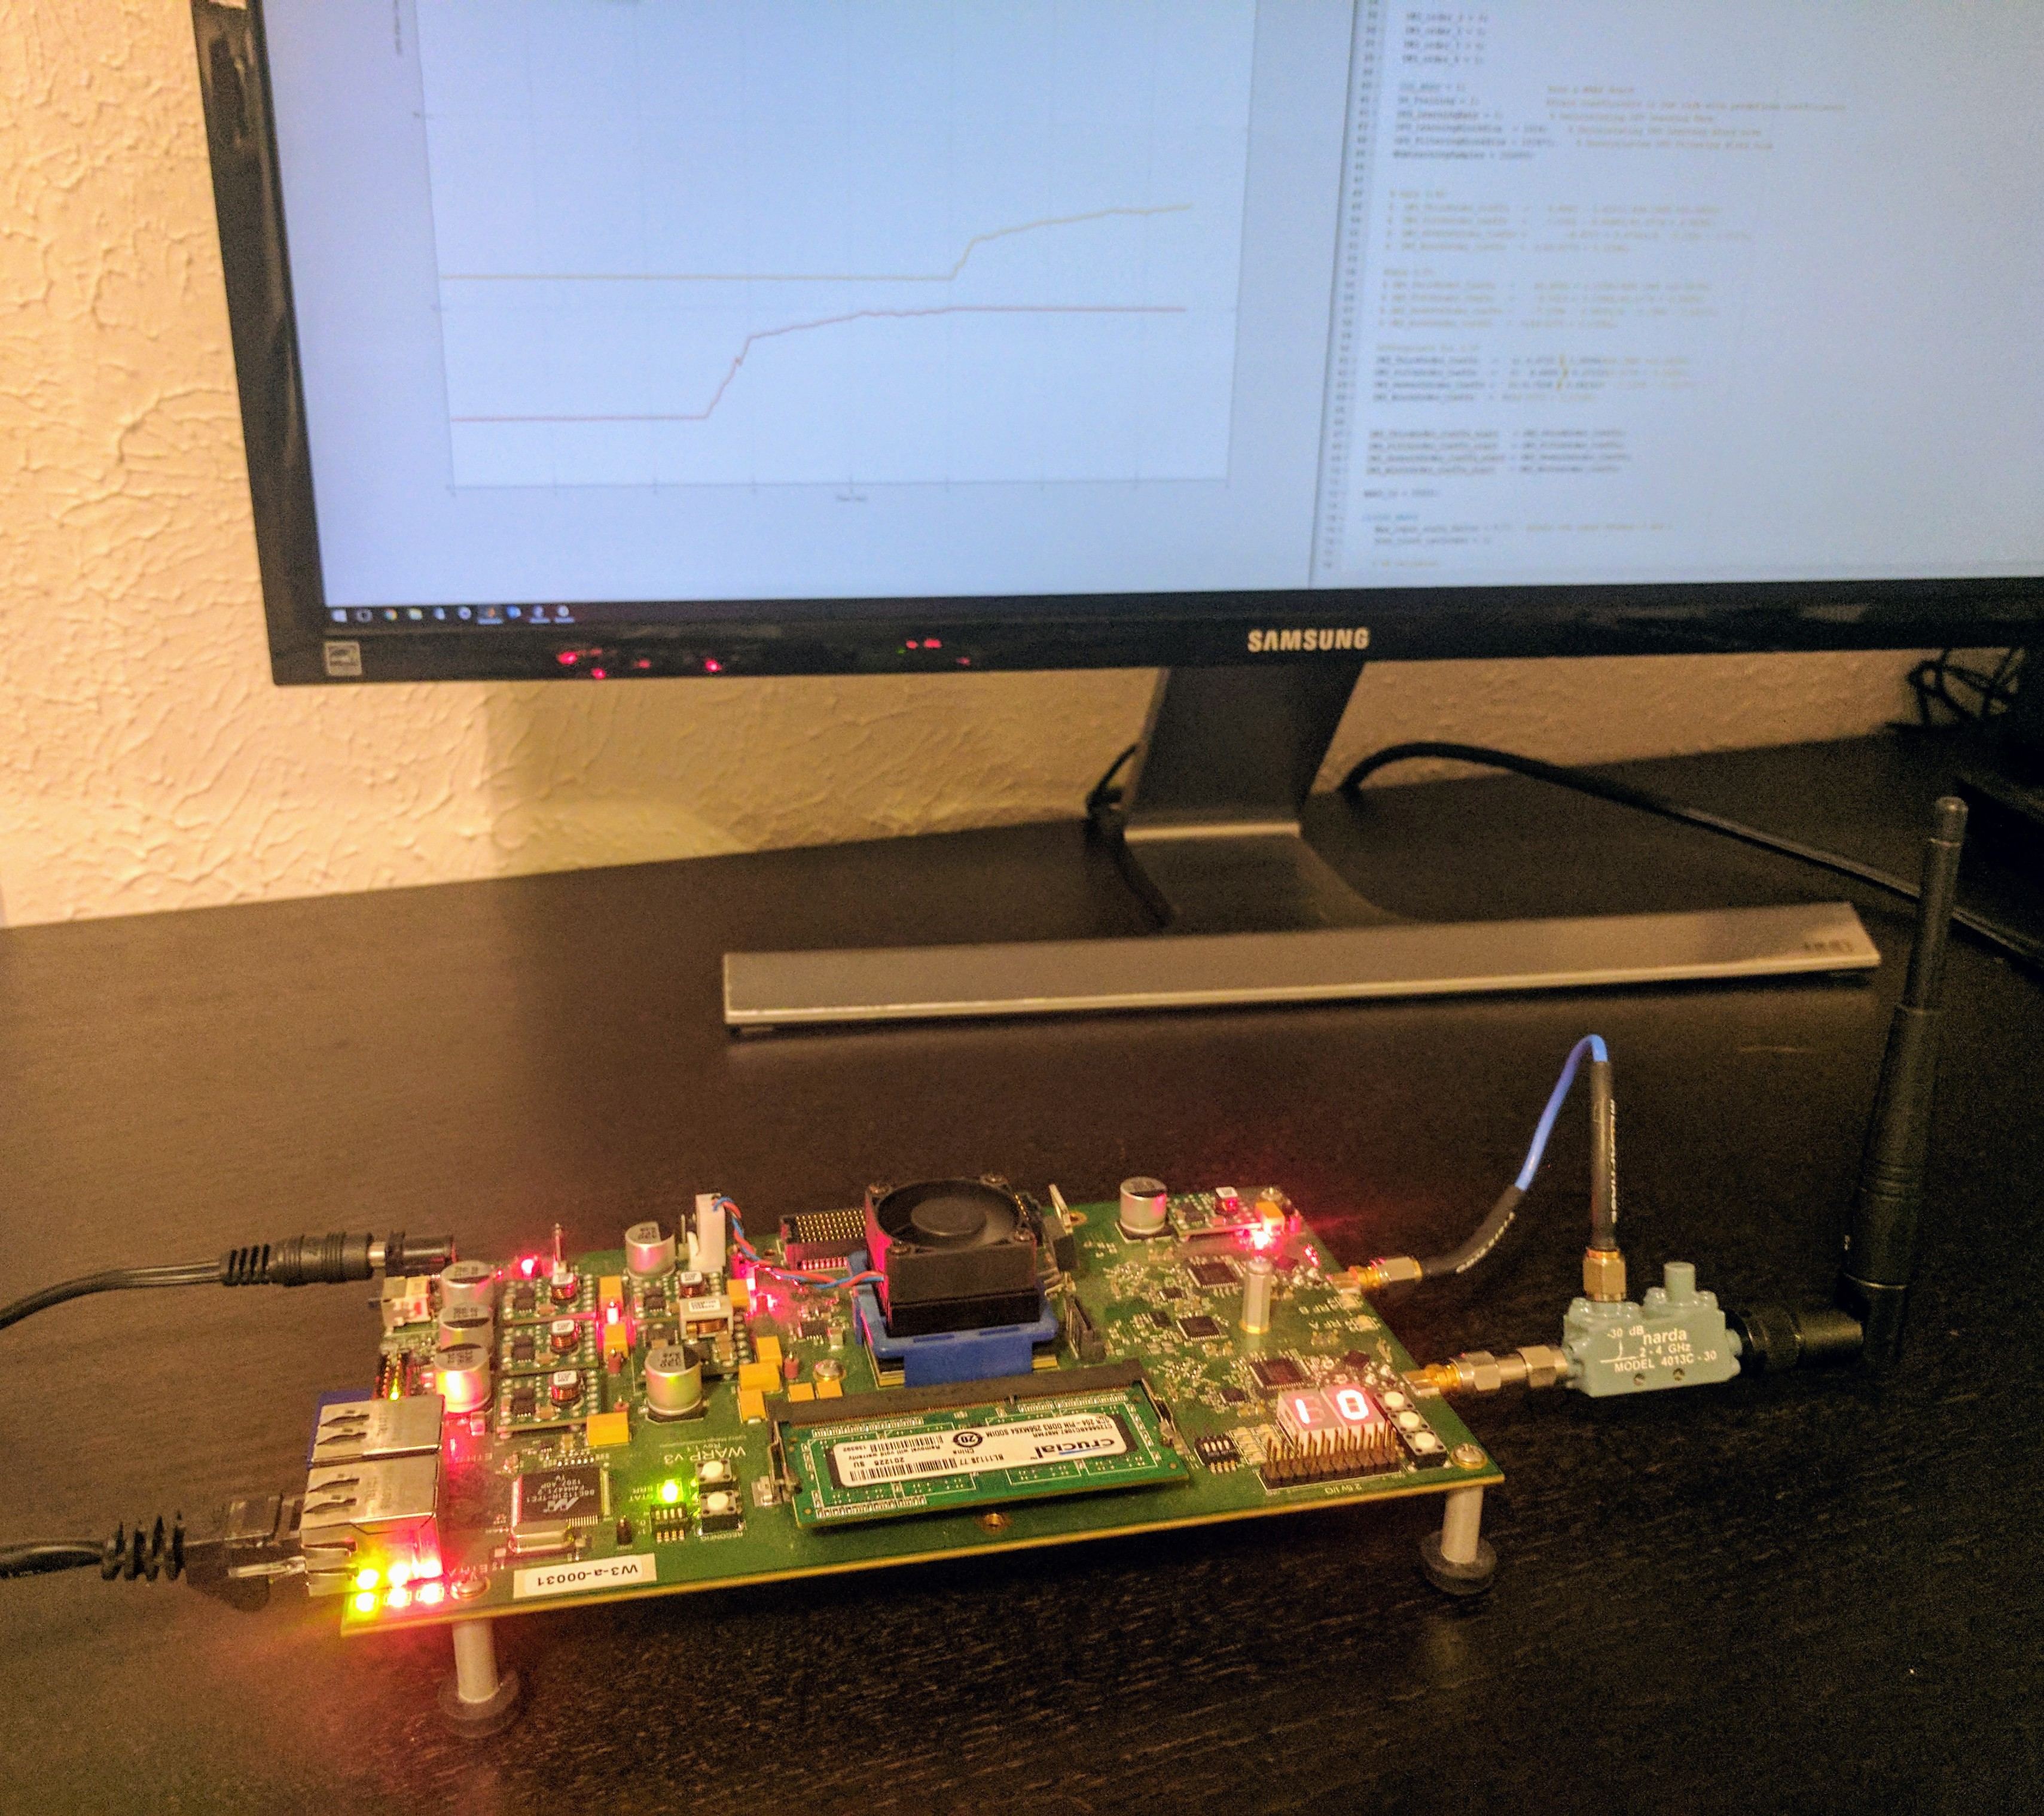
\includegraphics[width=0.75\columnwidth]{Figures/Setup.jpg}
\caption{The \textsc{Warp}v3 board interfaces with \textsc{Matlab} via an Ethernet cable connected to a PC. The TX port is directly connected to the RX port with 40 dB of inline attenuation for DPD training.}
\label{fig:exp_setup}
\end{figure}

\subsection{IM3$\pm$ Iterations}
We began by testing the iterative method presented in Section \ref{sec:Analysis}. 
An LTE uplink signal was generated in \textsc{Matlab} with two non-contiguous carriers. 
One carrier was 3 MHz and the other was 1.4 MHz. 
Both carriers had 64 QAM subcarrier modulation. 
The frequency domain results at each iteration are shown in Fig. \ref{fig:RightThenLeft}. 
The IM3+ spur was trained first using seventh-order DPD processing, and suppression was achieved as evident in the red curve. 
However, the IM3- spur magnitude was increased slightly which is consistent with (\ref{eq:IM3_-}). 
We then trained the IM3- spur (yellow curve). 
Again, there was a negative effect on the opposite spur, so we retrained the IM3+ spur (purple curve). 
At this point, we were satisfied with the performance and quit training. 

\begin{figure}[t!] 
\centering
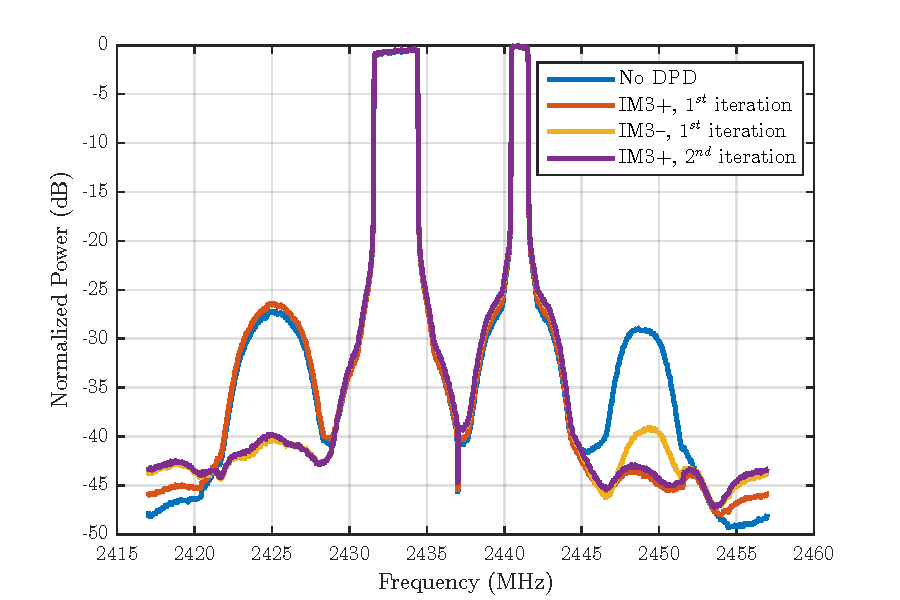
\includegraphics[width=0.9\columnwidth]{Figures/RightThenLeft_NEW}
\caption{Normalized spectral result when using the iterative method to suppress both the IM3+ and the IM3- spurs.}
\label{fig:RightThenLeft}
\end{figure}

\subsection{Sequential Learning}
As presented in Section \ref{sec:Sequential_Learning}, we then tested the sequential learning concept in \textsc{Warp}Lab where we started with low-order nonlinearities and added higher orders as needed. 
In Fig. \ref{fig:ConcurrentConvergence}, we show an example for comparison using the previously developed concurrent training method. 
We then switched to using the new sequential method as seen in Fig. \ref{fig:SequentialConvergence}. For these two experiments, the same LTE uplink signal and setup were used. 
We see that all the coefficients converged to approximately the same value. 
In Fig. \ref{fig:IterativeSpectrumvsConcurrent}, we show the results in the frequency domain on the IM3+ spur. 
From these figures, it is evident that the final result is equivalent and the only difference is the amount of time it takes to train.

\begin{figure}[t!] 
\centering
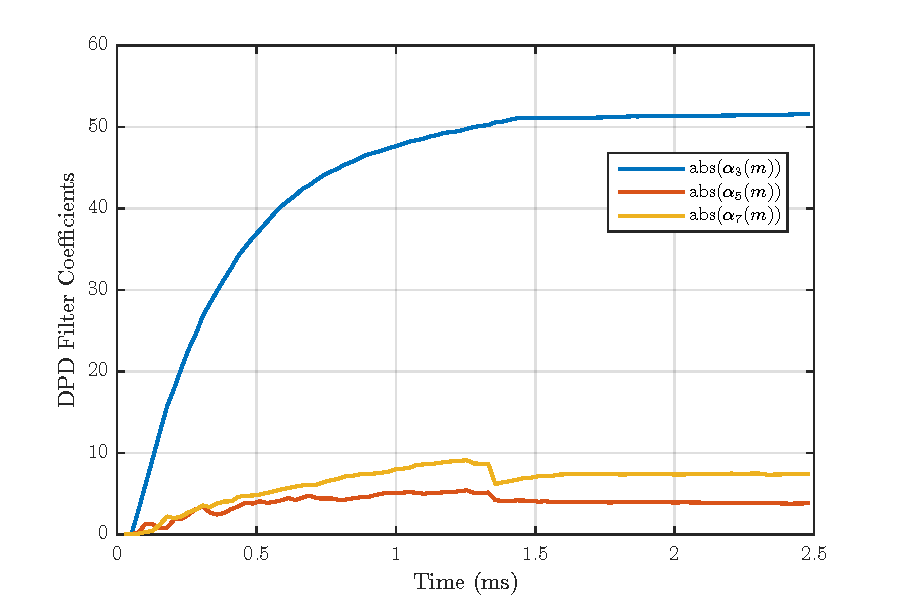
\includegraphics[width=0.9\columnwidth]{Figures/ConcurrentConvergence}
\caption{Example DPD coefficient convergence when concurrent training is used. 
	By training multiple orders concurrently, convergence occurs more rapidly at the price of additional hardware complexity when compared to sequential learning.}
\label{fig:ConcurrentConvergence}
\end{figure}

\begin{figure}
\centering
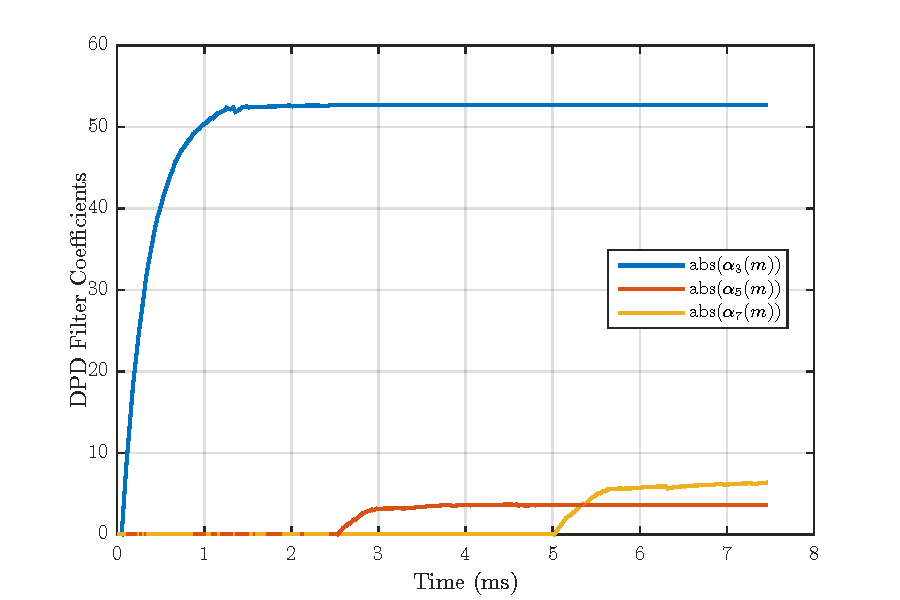
\includegraphics[width=0.9\columnwidth]{Figures/SequentialConvergence}
\caption{\textsc{Warp}Lab testing of sequential learning of DPD coefficients. 
	By training multiple orders sequentially, convergence occurs more slowly with the benefit of less hardware complexity when compared to concurrent learning.}
\label{fig:SequentialConvergence}
\end{figure}

\begin{figure}[t!] 
\centering
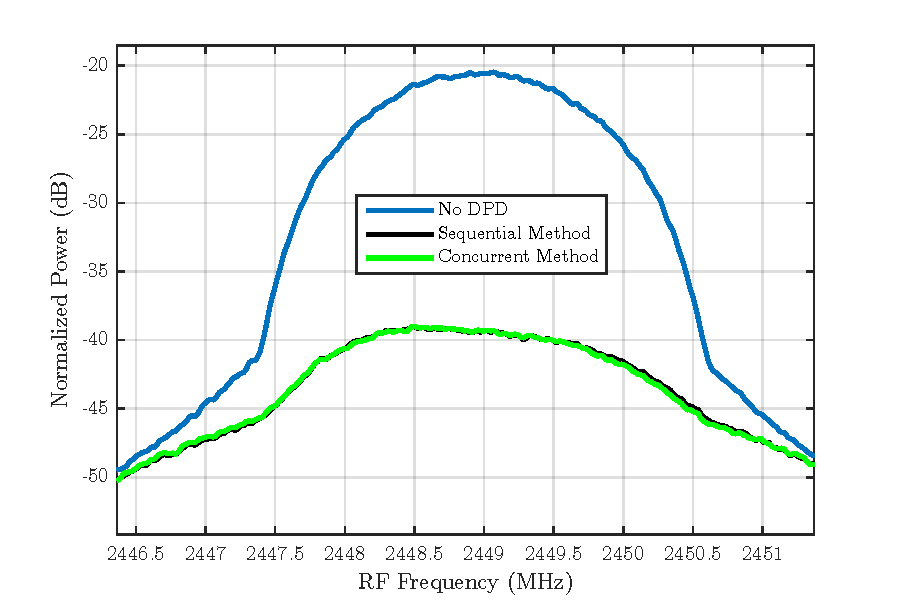
\includegraphics[width=0.9\columnwidth]{Figures/IterativeSpectrumvsConcurrent}
\caption{PSD result when using the concurrent and sequentially trained coefficients to suppress the IM3+ spur. 
	This shows nearly identical performance between the methods.}
\label{fig:IterativeSpectrumvsConcurrent}
\vspace{-10pt}
\end{figure}

\subsection{Speed-up Methods}
The convergence time for sequential training is longer than training in parallel as discussed earlier and shown in Figures \ref{fig:ConcurrentConvergence} and \ref{fig:SequentialConvergence}. 
To overcome this, we tested the previously presented methods for speeding up the convergence time.

We tested the adaptive $\mu$ concept presented by Algorithm 1. 
In Fig. \ref{fig:Convergence_Mu}, we show the correlation between the error block and the LMS reference block as the algorithm converges. 
As the DPD coefficient convergences (shown in blue), the correlation decreases (shown in orange). 
When it is below the threshold ($\gamma$) of 0.05 (shown in red) more than 5 times (the confidence metric, $\nu$), the learning rate changes from $\mu = 4$ to $\mu = 0.7$. 
This change of $\mu$ is denoted by the dashed line. 
The values were determined experimentally to what worked well for a variety of scenarios as determined by the authors. 

\begin{figure}[t!] 
\centering
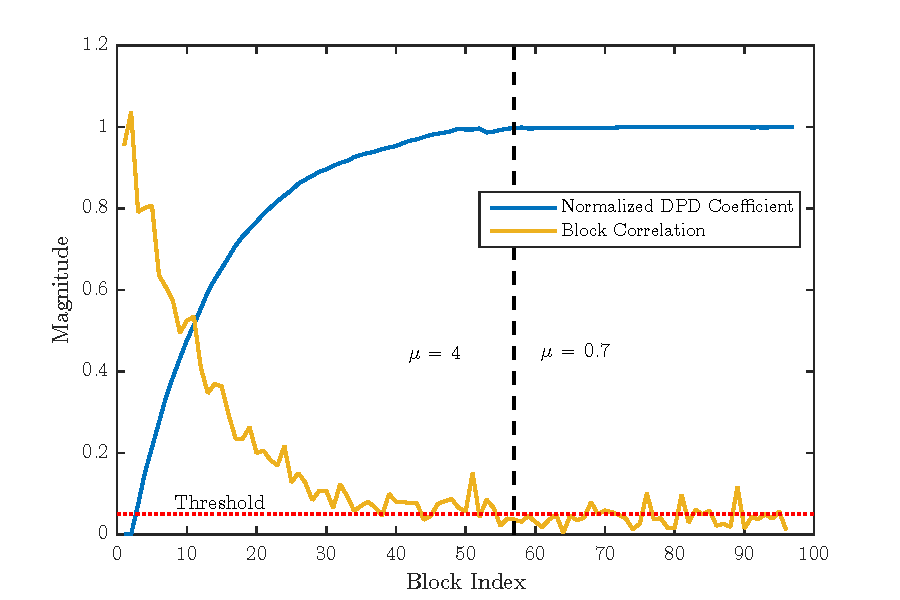
\includegraphics[width=0.9\columnwidth]{Figures/Convergence_Mu}
\caption{Correlation vs. block index during DPD training. 
	As training progresses the correlation decreases. 
	Once it is below the threshold for a total number of times greater than the confidence metric, we change to the lower learning rate.}
\label{fig:Convergence_Mu}
\vspace{-10pt}
\end{figure}

We then tested the concept of starting the DPD coefficient training from previous values. 
Using the same signal conditions as the experiment from Fig. 6, we increased the transmit power by approximately 2 dB.
 By doing so, we were operating in a more nonlinear region of the PA where we would have more distortion to overcome. 
 When we broadcasted at the new power levels, the need to retrain was apparent. 
 Without DPD, the IM3+ power was 20 dB lower than the main carriers. When using the final, converged coefficients from Fig. 6 that we obtained while training at a lower power at the new, higher transmit power, we still see suppression of the IM3+ spur. 
 However, it was only about 11 dB of suppression. 
 We then retrained but used the old, stale coefficients from Fig. 6 as a starting point. 
 By doing so, we were able to reduce the amount of time necessary for convergence by a factor of 2 and obtain approximately 20 dB of suppression. 
 The convergence of the coefficients from this experiment is shown in Fig. \ref{fig:UseOldCoeff_IncreasePower_Convergence}. 

\begin{figure}[t!] 
\centering
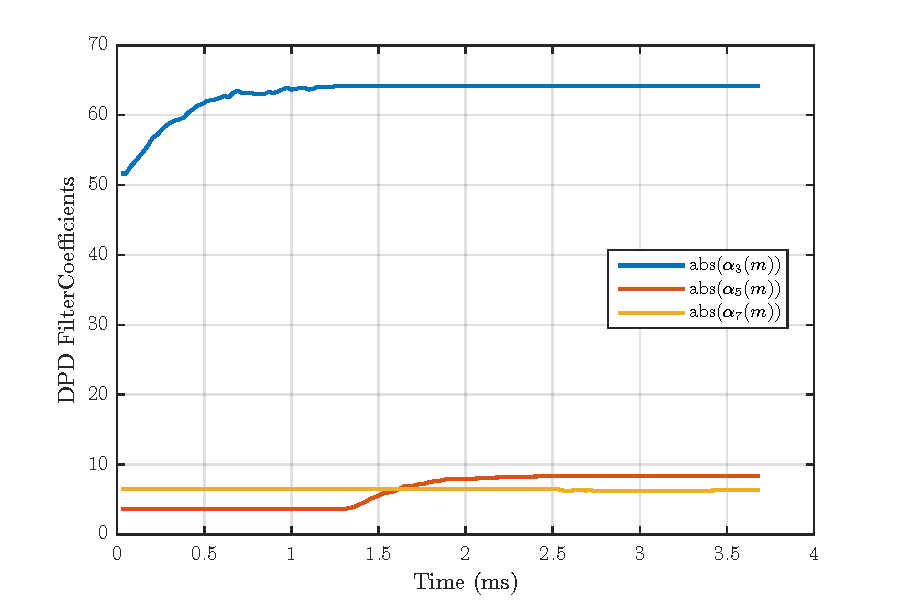
\includegraphics[width=0.9\columnwidth]{Figures/UseOldCoeff_IncreasePower_Convergence}
\caption{Convergence of the DPD coefficients when training starts at previously obtained coefficients.}
\label{fig:UseOldCoeff_IncreasePower_Convergence}
\vspace{-10pt}
\end{figure}

This concept can be further extended to include interpolating estimated DPD coefficients. As we store DPD coefficients for values, we build a table of DPD coefficients for varying PA gain parameters. Whenever we attempt to broadcast at a gain between two that are already in the table, we simply interpolate from the two. 



%\begin{figure}[t!] 
%\centering
%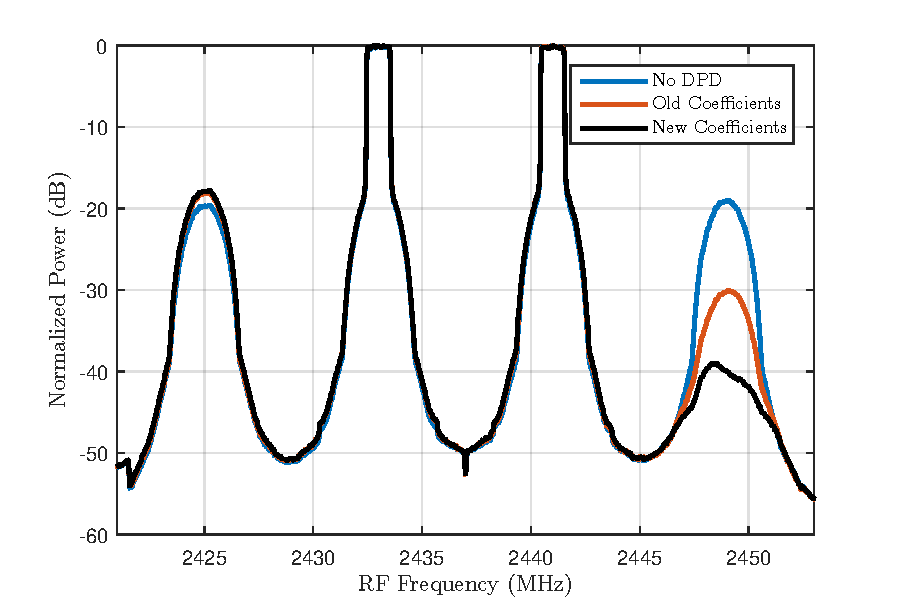
\includegraphics[width=\columnwidth]{Figures/UseOldCoeff_IncreasePower_PSD}
%\caption{}
%\label{fig:UseOldCoeff_IncreasePower_PSD}
%\end{figure}



